\documentclass[11pt,a4paper]{article}
\usepackage{a4wide}
\usepackage{amsmath}
\usepackage{amssymb}
\usepackage{amsfonts}
\usepackage{verbatim}
\usepackage{fancyvrb}
\usepackage{fixltx2e}
\usepackage[utf8]{inputenc}
%\usepackage[latin1]{inputenc}
\usepackage[T1]{fontenc}
\usepackage[spanish]{babel}
\usepackage{indentfirst}
\usepackage{fancyhdr}
\usepackage{latexsym}
\usepackage{lastpage}
\usepackage{caratula}
\usepackage[colorlinks=true, linkcolor=black]{hyperref}
\usepackage{calc}
\usepackage{alltt}
\usepackage{verbatim}
\usepackage{hyperref}
\usepackage{url}
\usepackage{graphicx, subfigure}
\usepackage{float}
\usepackage{algorithm}
\usepackage{algorithmic}
\floatname{algorithm}{Algoritmo}
\renewcommand{\listalgorithmname}{Lista de algoritmos}
\renewcommand{\algorithmicrequire}{\textbf{Entrada:}}
\renewcommand{\algorithmicensure}{\textbf{Salida:}}
\renewcommand{\algorithmicend}{\textbf{fin}}
\renewcommand{\algorithmicif}{\textbf{si}}
\renewcommand{\algorithmicthen}{\textbf{entonces}}
\renewcommand{\algorithmicelse}{\textbf{si no}}
\renewcommand{\algorithmicelsif}{\algorithmicelse,\ \algorithmicif}
\renewcommand{\algorithmicendif}{\algorithmicend\ \algorithmicif}
\renewcommand{\algorithmicfor}{\textbf{para}}
\renewcommand{\algorithmicto}{\textbf{hasta}}
\renewcommand{\algorithmicforall}{\textbf{para todo}}
\renewcommand{\algorithmicdo}{\textbf{hacer}}
\renewcommand{\algorithmicendfor}{\algorithmicend\ \algorithmicfor}
\renewcommand{\algorithmicwhile}{\textbf{mientras}}
\renewcommand{\algorithmicendwhile}{\algorithmicend\ \algorithmicwhile}
\renewcommand{\algorithmicloop}{\textbf{repetir}}
\renewcommand{\algorithmicendloop}{\algorithmicend\ \algorithmicloop}
\renewcommand{\algorithmicrepeat}{\textbf{repetir}}
\renewcommand{\algorithmicuntil}{\textbf{hasta que}}
\renewcommand{\algorithmicprint}{\textbf{imprimir}} 
\renewcommand{\algorithmicreturn}{\textbf{devolver}} 
\renewcommand{\algorithmictrue}{\textbf{cierto }} 
\renewcommand{\algorithmicfalse}{\textbf{falso }} 

\parskip = 11pt

% Pseudocódigo a lo Cormen
\usepackage{package/clrscode}

% auxiliares
\newcommand{\sisosi}{\Leftrightarrow}

\newcommand{\Frac}{\displaystyle\frac}

\newcommand{\suma}[2]{\sum\limits_{#1}^{#2}}

\newcommand{\Suma}[2]{\displaystyle\sum\limits_{#1}^{#2}}

\newcommand{\bc}{\begin{center}}
\newcommand{\ec}{\end{center}}


%\addtolength{\hoffset}{-1cm}
%\addtolength{\textwidth}{2cm}
 \addtolength{\voffset}{-0.5cm}
 \addtolength{\textheight}{1cm}
 
 %Datos de la caratula
\materia{Algorítmos y Estructura de Datos III}
\subtitulo{Algoritmos, complejidad, recursión}
\titulo{Trabajo Práctico 3}

\fecha{21 / 06 / 2013}
\integrante{Augusto Mascittija}{954/11}{mascittija@gmail.com}
\integrante{Catriel Omar D'Elía}{964/11}{catriel.delia@gmail.com}
\integrante{Julián Osías Jamardo}{769/08}{jamardo.julian@gmail.com}
\integrante{Patricio Capanna}{866/10}{patriciocapanna@gmail.com}


\newcommand{\real}{\mathbb{R}}
\newcommand{\nat}{\mathbb{N}}
\newcommand{\eme}{\mathcal{M}}
\newcommand{\emeh}{\widehat{\mathcal{M}}}
\newcommand{\ere}{\mathcal{R}}

%%%%%%%%% MACROS %%%%%%%%%
\urldef\wikiMakefile\url{http://es.wikipedia.org/wiki/Make}
\urldef\mnistURL\url{http://yann.lecun.com/exdb/mnist/}
\urldef\wikiHouseholder\url{http://en.wikipedia.org/wiki/QR_decomposition#Using_Householder_reflections}

%%%%%%%% FIN MACROS %%%%%%

\begin{document}

\thispagestyle{empty}
\maketitle
\tableofcontents

\newpage

\section*{Introducción}
\addcontentsline{toc}{section}{Introducción}
Este trabajo consta de tres problemas a resolver \textbf{Camiones Sospechosos},  \textbf{La Joya Del Río de La Plata} y \textbf{Rompecolores}, que fueron resueltos con \textit{técnicas de ordenamiento}, \textit{algorítmos golosos}, \textit{backtraking}, etc. En cada ejercicio se explica el algoritmo elegido para resolverlo, junto con el pseudo código del mismo, el cálculo de complejidad y el análisis correspondiente.

\section*{Ejercicio 1}
\addcontentsline{toc}{section}{Ejercicio 1}

En este ejercicio se nos pide un algoritmo mejor que O($n^2$) para devolver el dia en el cual de comenzar el inspector su trabajo le permita controlar la mayor cantidad de camiones, donde '$n$' es la cantidad de camiones.\\
Hay dos problemas ¿Como armamos los intervalos y cómo contamos en cada intervalo la cantidad de camiones?

\subsubsection*{Implementación}
\addcontentsline{toc}{subsubsection}{Implementación}

\emph{Cómo elegimos cada intervalo}

Una opción sería obtener el primer y último día de arrivo de camiones y por cada día comprendido entre ambos contar la cantidad de camiones que entran en el intervalo.\\
El problema con esta propuesta es que ahora el algoritmos depende no solo de la cantidad de camiones si no de la diferencia en dias de arribo entre el primero y último.
¿Es necesario recorrer tanto? o dicho de otra manera ¿Hace falta considerar todos los posibles días en que el inspector puede comenzar su trabajo?\\

Para visualizar mejor, hicimos un gráfico esquemático de tiempo en días. Cada intersección a la recta larga horizontal es un camión $C_i$ que llega en el día dado, donde $i$ es el orden. La llave de abajo representa el intervalo de tiempo donde el inspector se encontrará trabajando, aquí D es el intervalo en día dado al problema como dato y $t_i$ el día de comienzo del turno del inspector. Este es el valor buscado.\\ Veamos tres casos:\\


Si se empieza el turno en un día arbitrario, anterior a la llegada de un camión:\\
\includegraphics[scale=0.6]{imagenes/pre.png}\\
se controla del camión cero al cinco.

Si se empieza el turno en un día arbitrario entre dos camiones.\\
\includegraphics[scale=0.6]{imagenes/pos.png}\\
se controla el camión seis pero pierdo el cero.

Si se empieza el turno justo en la llegada de un camión.\\
\includegraphics[scale=0.6]{imagenes/cero.png}\\
se controla el camion cero y el seis.\\
Ahora $t_i = t_0 = C_0$

Vemos que de los tres casos el óptimo, mejor o igual al resto, es el que tiene al inspector comenzando el mismo día que la llegada de un camión. Por eso llamamos a $t_i$, $t_0$ y ahora se cumple que $0 \le i < k$ con $k$ el orden de llegada del último camión.

Tenemos entonces una cantidad de intervalos o de $t_i$ lineal con respecto a $n$. No decimos igual, porque hay algunas mejoras que se pueden agregar para que en algunos casos poder considerar menos que $n$ intervalos, pero sin embargo la relación sigue siendo lineal.

\emph{¿Cómo contamos los camiones en cada intervalo?}

Lo siguiente es para cada intervalo saber que cantidad de camiones el inspector revisa. Lo primero que a uno se le ocurre es algo como:

\begin{codebox}
\zi $c \gets 0$
\RComment cantidad de camiones
\zi \For $j \gets$ 0 \To $n$
\zi \Do
\zi   \If $C[j] < t_i + D$ 

\zi
\Then $c \gets c + 1$
\End
\End
\zi
\Return $c$
\end{codebox}

Con C un arreglo o lista de los días en los que llega cada camión - no necesariamente ordenada.\\
Pero esta forma de contar es lineal. Nada impide que $t_i + D$ sea mayor al ante último camión y por lo tanto por cada $t_i$ haríamos una cantidad $n - 1$ de operaciones, esto nos deja en un algoritmo O($n^2$).

Pero mirando el gráfico es claro que si puedo ubicar rápido cual es el último camion que llega justo antes que termine el turno del inspector, esto es si puedo hallar $max([j | C_j < t_i + D])$ con poco costo, se puede obtener la cantidad de camiones en una cantidad constante de pasos, mediante $c \gets j - i + 1$.\\
Lo único que necesitamos para hacer esto es que nuestros datos estén dispuestos de forma similar al gráfico, esto es que estén ordenados y luego poder encontrar ``rápido'' el máximo $j$.\\

Si nos construimos un arreglo en donde cada posición tenga el número de día de la llegada de un camión y además pedimos que esté ordenado, luego podemos buscar $j$ con una búsqueda binaria que cuesta O($log(n)$). Vamos a tener que hacer tantas busquedas binarias como intervalos posibles con lo cual la complejidad quedaría O($nlog(n)$), siempre y cuando ordenar el arreglo no nos lleve más, pero esto no es así dado que existen algoritmos de ordenamiento de exactamente esta complejidad.

\emph{Observaciones finales}

En realidad no es necesario recorrer todos los $t_i$ posibles. 
Basta con seguir hasta que $t_j + D >= C_k$ con $k$ el último de los camiones y $j$ el \emph{primero}\footnote{asumo que por día pueden llegar más de un camión.} de los camiones que cumple esto, porque es evidente que $\forall i, j < j$ la cantidad de camiones que caen en dicho intervalo es una sucesión monótona decreciente.

La búsqueda binaria que vamos a hacer tiene la particularidad que no busca un número particular, pues $t_i + D$ puede no ser un día en el que caiga camión alguno, si no el máximo de los valores menores a $t_i + D$. 

\begin{codebox}
\zi \Comment Requiere: $D \ge 1$ 
\Procname{\proc{dia-optimo}(V, D)}
\li \proc{ordenar}(V) \RComment O($n.log(n)$)
\li $c \gets 0$
\li $i \gets -1$
\li $k \gets 0$

\li \If $V[0] + D > V[\id{largo}(V)]$
\li 	\Then \Return $(0, \id{largo}(V))$
\li	\Else 

\li \Repeat \RComment O(n)
\li 	$i \gets i + 1$
\li	$j \gets $ \proc{lower\_bound}(V[i..\id{largo(V)}], V[i] + D - 1) \RComment O($log(n)$)
\li	\If $c < j - i$
\li		\Then $c \gets j - i$
\li		      $k \gets V[i]$
	\End
\li \Until $V[i] + D \le V[\id{largo}(V)]$ 
\li	\If $V[i] + D - 1 \ge V[\id{largo(V)}] \wedge c = j - i $
\li		\Then 
\li			$ c \gets c + 1$
		\End
\li \Return $(k, c)$
	\End


\RComment O($n.log(n)$)
\end{codebox}


\subsection*{Análisis}
\addcontentsline{toc}{subsection}{Análisis}

Producimos cuatro gráficos que sirven para mostrar que la cota téorica es apropiada.
La Fig: \ref{ej111} muestra la complejidad empírica del algorítmo $T(n)$. 
Una constante propuesta, que surgué de dividir a $T(n)$ por la cota propuesta, i.e $k(n) = T(n) / n.log(n) ) $. \\
También se grafica la cota teórica $f(n) = n.log(n)$ múltiplicada por un valor obtenido a partir de la tendencia de $k(n)$ cuando $n$ tiende a infinito. 
Este último valor surge de mirar la figura: \ref{ej112}.
En esta se aprecia que la misma ya varía poco y la curva que mejor ajusta es decreciente. 
Se elije seis $(6)$ como valor tendencial.

Que $k(n)$ sea decreciente de forma asintótica nos da seguridad que la cota propuesta es correcta. Los valores elevados para $n$ pequeños no solo surgen de que al haber valores más chicos la naturaleza aleatoria de la entrada es muy influyente, si no por que la notación $O(f(n))$ esconde que $T(n)$ puede ser:

\bc
$T(n) = k_1f(n) + k_2 f_2(n) + .. + k_j f_j(n) = k( f(n) + k'_2f_2(n) + .. + k'_jf_j(n)) \sisosi$\\
$T(n) / f(n) = k ( 1 + \frac{k'_2f_2(n) + .. + k'_jf_j(n)}{f(n)}) = k(n)$ 
\ec

Entonces para que la cota sea válida, toda función $f_j$ debe ser de igual o menor orden que $f(n)$. Pero esto es así si solo sí, la k(n) resultante es no creciente con asíntota en $k$. \\
Esta observación está corroborada en los gráficos.

Las figuras \ref{ej121} y \ref{ej122} muestran como $n.log(n)$ en algún momento alcanza y pasa a $T(n) / log(n) = l(n)$ y por lo tanto l(n) es sub linearitmética, probablemente lineal. \\
Muestra también como $6.n$ donde el seis es la constante burdamente seleccionada en las dos figuras anteriores se ajusta bastante bien a $l(n)$.


\subsection*{Imágenes}

    	\begin{center}
          \begin{figure}[H]
                \caption{Ejercicio 1 - a - 1}
        	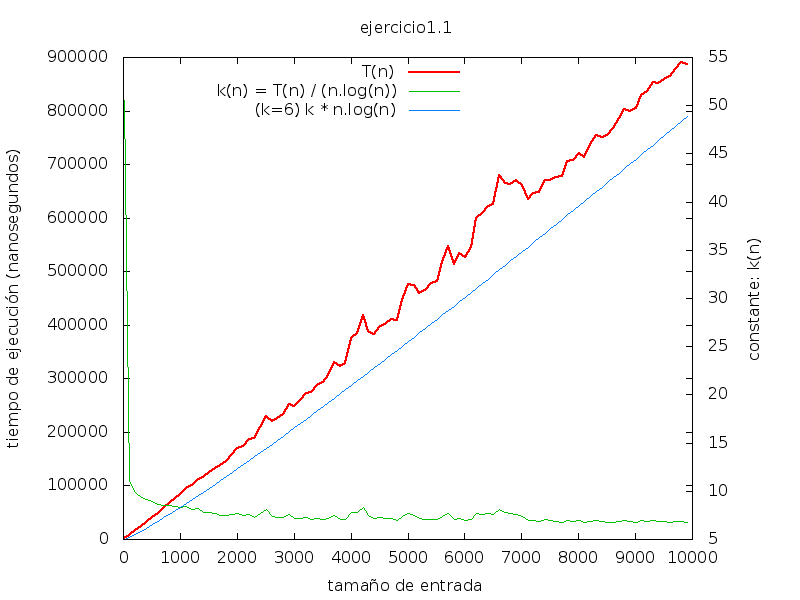
\includegraphics[scale=0.50]{imagenes/1-ejercicio1-1}
                \label{ej111}
          \end{figure}
    	\end{center}

    	\begin{center}
          \begin{figure}[H]
                \caption{Ejercicio 1 - a - 2}
        	\includegraphics[scale=0.50]{imagenes/1-ejercicio1-2}
                \label{ej112}
          \end{figure}
    	\end{center}

    	\begin{center}
          \begin{figure}[H]
                \caption{Ejercicio 1 - b - 1}
        	\includegraphics[scale=0.50]{imagenes/2-ejercicio1-2}
                \label{ej121}
          \end{figure}
    	\end{center}

    	\begin{center}
          \begin{figure}[H]
                \caption{Ejercicio 1 - b - 2}
        	\includegraphics[scale=0.50]{imagenes/1-ejercicio1-2}
                \label{ej122}
          \end{figure}
    	\end{center}



\section*{Ejercicio 2}
\addcontentsline{toc}{section}{Ejercicio 2}

En este problema tenemos que devolver un orden en el cual las piezas al ser fabricadas minimicen la pérdida de dinero del joyero por la devaluación del metal.\\
La complejidad que se nos pide es estrictamente menor a O($n^2$) con lo cual explorar todas las combinaciones no sirve pues es O($n!$).\\
La pregunta es ¿Qué usamos para ordenar?.
Intuitivamente podemos pensar que si el joyero fabrica las piezas que menos tiempo le llevan, tendrá menos pérdida, al acumulularse menos perdidas en el tiempo porque hay menos piezas pendientes.\\
Sin embargo con un simple contra ejemplo vemos que no es una elección que nos de una respuesta óptima.\\
\bc
$p_1 : (t_1 = 1, d_1 = 1)$\\
$p_2 : (t_2 = 3, d_2 = 9)$\\
$t_1 \le t_2  \Rightarrow$ $PM = [p_1, p_2]$\\
Sería la permutación buscada, y su costo:\\
$C(2, PM) = d_1t_1 + d_2(t_1+t_2) = 1 + 9*4 = 37$\\
Pero la permutación \\
$PM^* = [p_2, p_1]$\\
$C(2, PM^*) = d_2t_2 + d_1(t_1+t_2) = 3*9 + 1*4 = 31$\\
\ec
Es decir es más importante el precio y el algoritmo propuesto nos lleva a una permutación incorrecta. 

Viendo de nuevo un poco la fórmula de costo para dos piezas \ldots\\
\bc
$d_1t_1 + d_2(t_1+t_2)$
\ec
Si $t_1 = t_2 \Rightarrow t_1 < t_1 + t_2$ entonces conviene que $d_2 < d_1$.\\
Podríamos ordenar entonces solamente considerando el precio. \\
Es facil ver que tendríamos un problea similar, pero antes veamos un contrajemplo.
\bc
$p_1 : (t_1 = 1, d_1 = 1)$\\
$p_2 : (t_2 = 10, d_2 = 5)$\\
$PM = [p_2, p_1]$ es la permutación que arrojaría el algoritmo y su costo:\\
$C(2, PM) = d_2t_2 + d_1(t_1 + t_2) = 5*10 + 1(10+1) = 50 + 11 = 61$\\
Mientras que la permutación:\\
$PM^* = [p_1, p_2]$ tiene un costo de \\
$C(2, PM^*) = d_1t_1 + d_2(t_1 + t_2) = 1*1 + 5(10+1) = 1 + 55 = 56$\\
\ec

De hecho reordenando la fórmula de costo
\bc
$d_1$ $t_1 + d_2(t_1+t_2) = t_1(d_1+d_2) + t_2$ $d_2$
\ec
Lo cual nos dice que si los precios son todos iguales, conviene ordenar los tiempos de menor a mayor, que es lo que habiamos propuesto antes.\\
Entonces tenemos por un lado que tenemos que ordenar los precios de mayor a menor y por otro lado que los tiempos de menor a mayor, pero esto no siempre es posible, porque las piezas pueden tener ordenes arbitrarios y es poco probable que esto se pueda hacer siempre.\\
¿Cómo podemos mantener la idea?\\
Podemos usar el cociente $t_i/d_i$ para la pieza $i$ y ordenar según el mismo.\\
Veamos los dos ejemplos anteriores:\\
\bc
$t_1 / d_1 = 1$\\
$t_2 / d_2 = 3 / 9 = 1 / 3$\\
$t_2 / d_2 \le t_1 / d_1 $\\
entonces la permutación devuelta es la $[p_2, p_1]$ que es la óptima\\

y para el otro ejemplo...\\
$t_1 / d_1 = 1$\\
$t_2 / d_2 = 10 / 5 = 1 / 2$\\
$t_2 / d_2 \le t_1 / d_1 $\\
entonces la permutación devuelta es la $[p_2, p_1]$ que era la óptima\\
\ec

Es importante notar que la desigualdad, debe ser menor o igual y no menor estricta, si no se puede dar el caso de no poder ordenar el arreglo, por ejemplo:
\bc
$p_1 : (t_1 = 1, d_1 = 2)$
$p_2 : (t_1 = 5, d_2 = 10)$
\ec
Sería una entrada inválida si el algoritmo usara desigualdades estrictas. Relajemos está condición.\\
Las razones de $t / d$ dan lo mismo. Ahora nuestro criterio no permite distinguir entre ambas permutaciones, entonces surgue la siguiente pregunta. ¿Dan lo mismo los costos de ambas permutaciones?\\
Veamos:\\
\bc
$PM_1 = [p_1,p_2], PM_2 = [p_2, p_1]$\\
$C(2, PM_1) = 2*1 + 10*6 = 62 $\\
$C(2, PM_2) = 10*5 + 2*6 = 62 $\\ 
$C(2, PM_1) = C(2, PM_2)$
\ec
Aparentemente vamos bien encaminados.


\subsubsection*{Implementación}
\addcontentsline{toc}{subsubsection}{Implementación}

\begin{codebox}
\Procname{$\proc{Permutación-Con-Menor-Costo}(V)$}
\zi
  \Comment Calculamos los cocientes
\li $C \gets$ Arreglo($\id{largo}[V]$)
\li \For $i \gets 1$ \To $\id{largo}[V]$  \RComment O($n$)
\li   \Do
\li     $C[i] \gets (\id{V[i].tiempo} / \id{V[i].perdida-por-dia}, i) $  
     \End
     \RComment O(1)
\zi
  \Comment Ordenamos según el cociente de $C$
\li \proc{algun-algoritmo-de-ordenamiento}(C) \RComment O($n^2$) o O($nlog(n)$)
\li $R \gets  \id{Array[largo(C)]}$
\li \For $i \gets 1$ \To $\id{largo}[C]$ \RComment O($n$)
\li   \Do
\li     $R[i] \gets C[i].indice$
      \End
\li \Return $R$
\RComment O($n$) + O($n^2$) = O($n^2$) ó \zi
\RComment O($n$) + O($nlog(n)$) = O($nlog(n)$) \zi \RComment dependiendo del algoritmo de ordenamiento usado.
\end{codebox}

\subsection{Correctitud}

Tenemos un orden en que se fabricarán las piezas, esto es una permutación y queremos encontrar la que minimice costo.

Sean $t_i$, el tiempode fabricaci\'on, $d_i$ la perdida por día y $p_i$ la posición en la permutación de la $i$-esima pieza.

Sea $PM$ una permutaci\'on de las piezas en el orden de fabricaci\'on :

\bc
$PM = [p_1, p_2, \ldots , p_n]$
\ec

Como ya vimos, la ecuaci\'on de costos para una permitaci\'on es :

\bc
$C(n, PM) = d_1t_1 + d_2(t_1 + t_2) + \ldots + d_n(t_1 + t_2 + \ldots +t_n)$\\
\ec

Lo que tambi\'en se puede expresar en una formula cerrada como:

\bc
$\Suma{i=1}{n}(d_i \Suma{j=1}{i}t_j)$
\ec

\texttt{Por absurdo vamos a demostrar que si yo tengo una permutaci\'on \'optima no ordenada segun el cociente $t_i/d_i$ de sus piezas, de menor a mayor, puedo encontrar otra permutaci\'on cuya ecuaci\'on de costos sea menor a la ecuaci\'on de costos de la \'optima, con lo cual eso nos llevar\'ia al absurdo y el mundo puede colapsar.}

Entonces:

Sea PM una permutaci\'on \textbf{\'optima} con por lo menos dos elementos no ordeanados seg\'un nuestro criterio establecido.

Sean $p_i$, $p_{i+1}$ dos piezas consecutivas\footnote{No tienen por que ser consecutivas pero se toma as\'i para simplificar los indices en los c\'alculos.} de la permutaci\'on $PM$ que no cumplen el orden definido. Lo que quiere decir que $\frac{t_i}{d_i} > \frac{t_{i+1}}{d_{i+1}}$

Luego me genero una nueva permutaci\'on $PM^*$ exactamente igual a $PM$ salvo el orden de $p_i$, $p_{i+1}$. En esta nueva permutaci\'on estas dos piezas cumplen el orden pretendido.

\bc
$PM = [p_1, p_2, \ldots, p_i, p_{i+1}, \ldots , p_n$]\\
$PM = [p_1, p_2, \ldots, p_{i+1}, p_i, \ldots , p_n$]
\ec


Veamos entonces las ecuaciones de costos de cada una:

\bc
$C(n, PM) = d_1t_1 + d_2(t_1 + t_2) + \ldots + d_i\suma{j=1}{i}t_j + d_{i+1}\suma{j=1}{i+1}t_j + \ldots + d_n(t_1 + t_2 + \ldots +t_n)$\\
$C(n, PM^*) = d_1t_1 + d_2(t_1 + t_2) + \ldots + d_{i+1}(\suma{j=1}{i-1}t_j + t_{i+1})+ d_i(\suma{j=1}{i+1}t_j)  + \ldots + d_n(t_1 + t_2 + \ldots +t_n)$\\
\ec

Como \textbf{PM} es una permutaci\'on \'optima entonces :

\bc
$C(n, PM) - C(n,PM^*) \le 0$\\
$\sisosi$\\
$ d_i\suma{j=1}{i}t_j + d_{i+1}\suma{j=1}{i+1}t_j - (d_{i+1}(\suma{j=1}{i-1}t_j + t_{i+1})+ d_i\suma{j=1}{i+1}t_j) \le 0$\\
$\sisosi$\\
$d_{i}(\suma{j=1}{i}t_j - \suma{j=1}{i+1}t_j) + d_{i+1}(\suma{j=1}{i+1}t_j - \suma{j=1}{i-1}t_j + t_{i+1}) \le 0$\\
$\sisosi$\\
$d_{i+1}$ $t_i - d_i$ $t_{i+1}$ $\le 0$\\
$\sisosi$\\
$d_{i+1}$ $t_i \le d_i$ $t_{i+1}$\\
$\sisosi$\\
$\frac{t_i}{d_i} \le \frac{t_{i+1}}{d_{i+1}}$\\
\ec

Lo cu\'al es \textsc{absurdo}, pues $\frac{t_i}{d_i} > \frac{t_{i+1}}{d_{i+1}}$. Y el absurdo provino de suponer que la permutaci\'on $PM$ es \'optima y no est\'a ordenada de menor a mayor segun $\frac{t_i}{d_i}$.\\


\subsection*{Análisis}
\addcontentsline{toc}{subsection}{Análisis}

Producimos cuatro gráficos que sirven para mostrar que la cota téorica es apropiada.
La Fig: \ref{ej211} muestra la complejidad empírica del algorítmo $T(n)$. 
Una constante propuesta, que surgué de dividir a $T(n)$ por la cota propuesta, i.e $k(n) = T(n) / n.log(n) ) $. \\
También se grafica la cota teórica $f(n) = n.log(n)$ múltiplicada por un valor obtenido a partir de la tendencia de $k(n)$ cuando $n$ tiende a infinito. 
Este último valor surge de mirar la figura: \ref{ej212}.
En esta se aprecia que la misma ya varía poco y la curva que mejor ajusta es decreciente. 
Se elije nueve $(9)$ como valor tendencial.

Que $k(n)$ sea decreciente de forma asintótica nos da seguridad que la cota propuesta es correcta. Los valores elevados para $n$ pequeños no solo surgen de que al haber valores más chicos la naturaleza aleatoria de la entrada es muy influyente, si no por que la notación $O(f(n))$ esconde que $T(n)$ puede ser:

\bc
$T(n) = k_1f(n) + k_2 f_2(n) + .. + k_j f_j(n) = k( f(n) + k'_2f_2(n) + .. + k'_jf_j(n)) \sisosi$\\
$T(n) / f(n) = k ( 1 + \frac{k'_2f_2(n) + .. + k'_jf_j(n)}{f(n)}) = k(n)$ 
\ec

Entonces para que la cota sea válida, toda función $f_j$ debe ser de igual o menor orden que $f(n)$. Pero esto es así si solo sí, la k(n) resultante es no creciente con asíntota en $k$. \\
Esta observación está corroborada en los gráficos.

Las figuras \ref{ej221} y \ref{ej222} muestran como $n.log(n)$ en algún momento alcanza y pasa a $T(n) / log(n) = l(n)$ y por lo tanto l(n) es sub linearitmética, probablemente lineal. \\
Muestra también como $9.n$ donde el seis es la constante burdamente seleccionada en las dos figuras anteriores se ajusta bastante bien a $l(n)$.


\subsection*{Imágenes}

    	\begin{center}
          \begin{figure}[H]
                \caption{Ejercicio 2 - a - 1}
        	\includegraphics[scale=0.50]{imagenes/1-ejercicio2-1}
                \label{ej211}
          \end{figure}
    	\end{center}

    	\begin{center}
          \begin{figure}[H]
                \caption{Ejercicio 2 - a - 2}
        	\includegraphics[scale=0.50]{imagenes/1-ejercicio2-2}
                \label{ej212}
          \end{figure}
    	\end{center}

    	\begin{center}
          \begin{figure}[H]
                \caption{Ejercicio 2 - b - 1}
        	\includegraphics[scale=0.50]{imagenes/2-ejercicio2-2}
                \label{ej221}
          \end{figure}
    	\end{center}

    	\begin{center}
          \begin{figure}[H]
                \caption{Ejercicio 2 - b - 2}
        	\includegraphics[scale=0.50]{imagenes/1-ejercicio2-2}
                \label{ej222}
          \end{figure}
    	\end{center}



\section*{Ejercicio 3}
\addcontentsline{toc}{section}{Ejercicio 3}

En este ejercicio, se tiene un tablero de $nxm$ posiciones, y $nxm$ piezas para ubicar en estos casilleros. Las piezas son cuadradas y puede tener hasta cuatro colores en cada uno de sus lados ($inferior$, $superior$, $izquierda$ y $derecha$). El objetivo es ubicar las piezas en el tablero de manera que entre dos piezas adyacentes, los lados que se tocan, deben ser iguales.
Un punto importante a tener en cuenta es que no es necesario ubicar todas las piezas en el tablero, dejar una posición en blanco es totalmente válido, por lo que, la mejor solución será aquella que logra ingresar la mayor cantidad de piezas en el tablero.
Para esto, se pide utilizar la técnica de backtraking. El algoritmo consiste en ir tomando soluciones parciales formando una especie de árbol. Se van recorriendo las ramas hasta llegar a las soluciones (hojas del árbol) y o bien se detiene, o bien se vuelve sobre la rama para buscar nuevas soluciones. Para ejemplificar, en un tablero de 3 posiciones con las piezas $1$, $2$ y $3$, donde la única posible solución es la combinación $1$, $3$, $2$, el árbol quedaría de la siguiente manera:

	\begin{figure}[H]
    	\begin{center}
        	\includegraphics[scale=0.50]{imagenes/arbol_basico.png}
    	\end{center}
    	\caption{Arbol Backtraking}
    	\label{fig:arbol_basico}
	\end{figure}

Si a este árbol agregamos la pieza vacía (a lo largo del trabajo la denotaremos con el valor $-1$) habría que agregar todas las ramas que la contemplen desde el inicio.

\subsection*{Implementación}
\addcontentsline{toc}{subsection}{Implementación}

El problema básicamente consta en ir obteniendo piezas y ubicándolas en un tablero de $n$ filas por $m$ columnas, utilizando el método \textbf{backtraking}.
Para resolverlo, se recorre el tablero por \textbf{filas}, de \textit{izquierda a derecha} lógicamente, empezando en la posición $(1,1)$ y finalizando en la posición $(n,m)$.

El algoritmo más sencillo de backtraking implementado, toma como parámetros de entrada la posición $(i,j)$ en la que queremos ubicar la pieza, con un ciclo principal que itera sobre una lista de piezas disponibles (aquellas que todavía no fueron ubicadas en ninguna posición del tablero). En cada iteración va a consultar si la pieza se puede ubicar y en el caso de que fuera posible, se realiza el llamado recursivo con la próxima posición del tablero que necesitamos completar. Cuando dentro del ciclo, se retorna del llamado recursivo, entonces debemos probar con la próxima pieza en esa posición, es decir, seguimos con el próximo paso de la iteración.
Como se comentó anteriormente es necesario tomar en cuenta la posibilidad de dejar espacios en blanco en el tablero, por lo que, cuando la iteración termina, se hace el llamado recursivo con la próxima posición dejando esa vacía.
La mejor solución se guarda cuando el número de piezas ubicadas en el tablero, es mayor que el número de piezas de la mejor solución que tenemos guardado.

A continuación se expone un pseudocódigo muy simple, con el fin de mostar como funciona el algoritmo en su versión más básica.

\begin{Verbatim}[commandchars=\\\{\}]
rompecolores(fila, columna) : (requiere fila >= 0, columna >= 0)

	* Si columna > m && fila > n
		* retornar
	
	* Para cada pieza disponible :
		* Si not(llenarPosicion(fila, columna))
			* continuar iteracion.
		* fin Si
		* numPiezasUbicadas++
		* Si numPiezasUbicadas > numPiezasMejorSolucion
			* numPiezasMejorSolucion = numPiezaUbicadas
			* guardarMejorSolucion()
		* fin Si
		* rompecolores(proxima(fila), proxima(columna))
		* vaciarPosicion(fila, columna)
		* numPiezasUbicadas--
	* fin Para
	
	rompecolores(proxima(fila), proxima(columna))
fin
\end{Verbatim}

Es importante aclarar que en la implementación real, tanto el tablero, la lista de piezas, el contador numPiezasUbicadas y numPiezasMejorSolucion son variables accesibles por el algoritmo de manera que en cada llamado recursivo, tienen los valores actualizados.
La función \textbf{llenarPosicion} se encarga de probar la pieza en la posición $(fila, columna)$, si se puede ubicar retorna \textit{true} y en caso contrario \textit{false}.

De esta manera, si la pieza se pudo ubicar hacemos el llamado recursivo para la próxima posición del tablero (notar que la función \textit{proxima}, que toma fila y columna, retorna la próxima posición valida del tablero) y si no, seguimos con la iteración, es decir, probamos la próxima pieza.
Por otro lado, la función \textbf{vaciarPosicion} libera la posición del tablero analizada, devolviendo la pieza a la lista de disponibles.

Notar que cuando la iteración termina, se realiza el llamado recursivo, dejando esa posición vacía (o mejor dicho, con una pieza en blanco).

Como se puede apreciar, el algoritmo termina cuando el tablero se termina, es decir, cuando columna y fila se van de rango, para un tablero de $nxm$ esto es, cuando $columna > m$ y $fila > n$, es decir, cada rama del backtraking se corta cuando llegamos al final del tablero.

\subsubsection*{Llenar y vaciar posición}
\addcontentsline{toc}{subsubsection}{Llenar y vaciar posición}
La manera que se llena la posición dependerá del algoritmo implementado. Como se aprecia, la función rompecolores consta de un ciclo principal sobre la cantidad de piezas disponibles. La tarea de ir probando las piezas se delega a un objeto llamado AutoFill  probará una pieza, en caso de poder utilizarse, se ubicará en el tablero y retornará true y en caso contrario, la ubicará al final de la lista de piezas por ubicar, para que en el próximo llamado, es decir, en el próximo paso de la iteración pruebe con otra.

En términos de implementación y sólo para mencionarlo, AutoFill se podría comparar con el patrón "strategy". Existen dos maneras de ejecutar el algoritmo, la forma \textbf{básica} y la forma \textbf{mejorada}, llamados Basic AutoFill y Enhanced AutoFill respectivamente. Estas son las estrategias posibles para AutoFill, es decir, el básico y el mejorado, se comportan polimórficamente, de manera que el algoritmo es exactamente igual en ambos casos, lo que se modifica es cómo se llenan y vacían las posiciones del tablero.

El llenado, en su versión básica, cómo se recorre de izquierda a derecha, sólo es necesario verificar la coincidencia entre el color de la izquierda de la pieza a ubicar y el de la derecha de la posición anterior, en caso de que no nos encontremos en la primera columna o sea una ficha blanca, y el color superior contra el inferior de la pieza ubicada inmediatamente arriba, también en caso de que exista, o no sea blanca.

Sin embargo, en la versión mejorado, se utilizan los colores para definir las posibles próximas piezas. Cuando se cargan las piezas, se van ubicando en un array bidimensional de $CxC$ con $C$ cantidad de colores, que contiene listas. Este array bidimensional representa los colores de la izquierda y superior. En cada posición del array se encuentra una lista de las piezas disponibles. Cuando llega el momento de ubicar una pieza nueva, como en el caso anterior, con el color inferior de la pieza superior y el color derecho de la pieza izquierda, podemos ingresar al array en O(1) y tomar el frente de la lista que se encuentra en esa posición y retornar true, o en su defecto, si no hay elementos en esa posición, es decir, no tenemos piezas retorna false.  De esta manera, podemos iterar en menos cantidad de piezas, ya que la mejora permite sólo iterar en aquellas piezas que se pueden ubicar y no en todas como sucede con el algoritmo básico.

\subsubsection*{Poda}
\addcontentsline{toc}{subsubsection}{Poda}
El agoritmo anterior, es la implementación más básica utilizando backtraking. Una buena idea para mejorarlo es "podar" aquellas ramas en la ejecución del algoritmo que ya no nos interesan. Definir que rama nos interesa y que rama no, es bastante sencillo, la intención es cortar la ejecución cuando el continuar por ese camino, no nos entregue una mejor solución.
Supongamos que tenemos 6 posiciones, por lo tanto, 6 piezas y la mejor solución que tiene almacenada el algoritmo consta de 4 piezas, pero, en la rama que estamos recorriendo sólo se pudieron ubicar 2 piezas y queda por analizar sólo una posición del tablero. Está claro que por más que a la última posición se le asigne una pieza, esta solución constará de 3 piezas y no es mejor que la que teníamos de 4, por lo que no es conveniente seguir por este camino.
Además, si supieramos la máxima cantidad de piezas que podríamos colocar, lograríamos refinar aún más el criterio. Por ejemplo, si en el ejemplo anterior, en lugar de quedar sólo una posición, quedaran dos, sería posible encontrar una solución de cuatro piezas, pero, si a priori uno supiera que la cantidad de piezas máximas que puede ubicar es una, entonces tampoco sería conveniente continuar por esa rama.

El Enhanced AutoFill, no solo determina que ficha se puede ubicar mejorando el número de iteraciones sino que, también basado en los colores, retorna cual es la máxima cantidad de fichas que se pueden ubicar siguiendo por esa rama. Tanto el básico como el mejorado implementan la función maximaCantPiezasEnTablero, solo que el primero, retorna la cantidad de piezas disponibles, mientras que el segundo lo que se comentó anteriormente.

\textit{Lo interesante de la solución propuesta, es que la poda se comporta de la misma manera sea cual sea la estrategia seleccionada para llenar las posiciones y calcular la cantidad de piezas por ubicar.
}
El siguiente pseudocódigo muestra la poda agregada:

\begin{Verbatim}[commandchars=\\\{\}]
rompecolores(fila, columna) : (requiere fila >= 0, columna >= 0)

	* Si columna > m && fila > n
		* retornar
	
	* Para cada pieza disponible :

		* Si not(llenarPosicion(fila, columna))
			* continuar iteracion.
		* fin Si

		* numPiezasPorUbicar = maximaCantPiezasEnTablero()
		* numPosicionesAnalizadas++
		* numPiezasUbicadas++

		* Si numPiezasUbicadas > numPiezasMejorSolucion
			* numPiezasMejorSolucion = numPiezaUbicadas
			* guardarMejorSolucion()
		* fin Si

		* Si poda_habilitada
			* var numPosicionesRestantes =
				numPosicionesTablero - numPosicionesAnalizadas
			* var posibilidades =
				min(numPosicionesRestantes, numPiezasPorUbicar)
			* Si ((posibilidades + numPiezasUbicadas) <= numPiezasMejorSol)
				* vaciarPosicion(fila, columna)
				* numPiezasPorUbicar = maximaCantPiezasEnTablero()
				* numPiezasUbicadas--
				* numPosicionesAnalizadas--
				* retornar
			* fin Si
		* fin Si	

		* rompecolores(proxima(fila), proxima(columna))
		* vaciarPosicion(fila, columna)
		* numPiezasPorUbicar = maximaCantPiezasEnTablero()
		* numPiezasUbicadas--
		* numPosicionesAnalizadas--

	* fin Para
	
	numPosicionesAnalizadas++	
	rompecolores(proxima(fila), proxima(columna))
	numPosicionesAnalizadas--

fin
\end{Verbatim}

En este caso, se agregan varios contadores para poder determinar cuando podar. La variable \textbf{numPiezasPorUbicar} contiene la máxima cantidad de piezas que se pueden ubicar en el tablero y se actualiza con la función \textbf{maximaCantPiezasEnTablero} luego de cada vez que se aplica \textbf{llenarPosicion} o \textbf{vaciarPosicion}. \textbf{numPosicionesAnalizadas} como indica su nombre, contiene el número de posiciones analizadas, tanto las que tienen piezas, como las que quedaron en blanco y \textbf{numPosicionesTablero} es el número total de posiciones, es decir $n * m$.

La función maximoCantPiezasEnTablero(), es básicamente la encargada de afinar el podado, y tiene sentido cuando el argumento --mejorar se encuentra presente. De lo contrario, cuando no se encuentra, maximoCantPiezasEnTablero es simplemente la cantidad de piezas restantes que siempre va a ser mayor o igual a la cantidad de numPosicionesRestantes, ergo no tiene importancia en ese caso.

Lo que calcula esta función es: Cantidad de espacios del tablero que me quedan menos cantidad de piezas que seguro no voy a poder poner. Y como probablemente intuyan, lo importante de esto es cómo se calcula aquella cantidad que seguro no puedo poner. 
En principio la idea es entender que hay una cantidad determinada de espacios en mi tablero (los cuales todavía no recorrí, y podría poner fichas) tal que tengo alguna información al respecto, y otros sobre los cuales decimos "no se nada". Catalogo a aquellos que "no se nada" como todos los espacios(una ubicacion en el tablero vacia) que no están en contacto con ninguna pieza, entiéndase contacto a que si me muevo un espacio horizontal o verticalmente me encuentro con una pieza puesta. El resto digo que tengo algo de información.


¿Cómo analiza la información el algoritmo mejorado la información? Lo que hacemos es diferenciar todas piezas por el color que tienen a su izquierda, luego por el color que tienen arriba, y finalmente por ambos colores al mismo tiempo. De esta manera tengo distinguidas todas las posibles combinaciones de piezas que puedo llegar a necesitar (esto se debe a que el algoritmo inserta piezas avanzando a la siguiente fila luego de haber completado todas las columnas de izquierda a derecha de una fila determinada). De hecho también voy a tener la cantidad que tengo de cada combinación.
En principio se nos ocurrió que la función distinga que fichas que no puede poner a partir de la siguiente secuencia de eventos:
1-Coloco una ficha
2-Chequeo en todos sus lados válidos (abajo si no estoy en la ultima fila, y derecha si no estoy en la última columna): Existe una pieza tal que puedo ponerlo en esta posición? (esto puedo saberlo si la cantidad de piezas que tengo de esas características IZQ Y ARR son las que necesito)
2.1- Si existe no hago nada
2.2- Si esta pieza no existe disminuyo el maximoPiezasPosibles

Luego caímos en cuenta de que quizás podríamos tener más información todavía. Ej. si tengo una secuencia de piezas tal que todas necesitan una pieza adyacente arriba con algún color especifico, digamos rojo. En este caso quizás tengo sólo 1 pieza que lo cumpla. Luego SE que SEGURO no voy a poder poner 2 piezas.
A partir de la idea agregamos a la estructura contenedora de piezas de un cierto tipo(color arriba y color izquierda), no sólo la cantidad de tal tipo, sino un campo cantidadRequerida. La misma representa como su nombre lo dice cuantas piezas están requiriendo a fin de estar conectadas esa combinación de color específica.
Si bien parece por ahora todo muy feliz. La solución no termina siendo tan feliz. La razón es que tenemos que tener en cuenta que cuando se requieren piezas del lado izquierdo de un cierto tipo pueden o no requerirse también piezas del lado de arriba. A veces 1 sola a veces ambas. Y la intersección de ambas hace difícil la decisión de cuando disminuyo el máximo de posibilidades. Encontramos que hay dos maneras de decrementar los que no puedo poner. 
1. Como el ejemplo, cuando tengo requerimientos de un sólo lado. En este caso se resuelve igual, me fijo cuantos requieren menos la cantidad que tengo.
2. Cuando tengo la combinación de algo requerido por la pieza de arriba más la de una pieza de la izquierda. En este caso descuento si la cantidad requerida de la combinación es mayor a la cantidad. Aunque si esto no sucede, es que tengo fichas iguales o de sobra a las requeridas, entonces lo trato como una pieza que tiene el requerimiento por arriba solamente. 

En sí la implementación no es tan feliz pero acota mucho más fino que el primer intento. 

Un dato importante de esta poda es que podemos obtener una información en general igual a m(columnas), esto es para tableros que sean de la forma n>1 por m. Como la información nos ayuda a acotar más la cantidad de piezas que podría poner, nos conviene que m sea mas grande que n. Esto se debe claro a la forma en la que inserto las piezas.
Entonces una posible mejora a la poda es girar el tablero cuando n>m. Y esto tiene un costo de O(n).

Extrayendo la sección del código que realiza la poda:

\begin{Verbatim}[commandchars=\\\{\}]
* Si poda_habilitada
	* var numPosicionesRestantes =
		numPosicionesTablero - numPosicionesAnalizadas
	* var posibilidades =
		min(numPosicionesRestantes, numPiezasPorUbicar)
	* Si ((posibilidades + numPiezasUbicadas) <= numPiezasMejorSol)
		* vaciarPosicion(fila, columna)
		* numPiezasPorUbicar = maximaCantPiezasEnTablero()
		* numPiezasUbicadas--
		* numPosicionesAnalizadas--
		* retornar
	* fin Si
* fin Si	
\end{Verbatim}

En esta sección del pseudocódigo logramos que si las posiciones restantes más el número de piezas ubicadas es menor o igual que la cantidad de piezas en la mejor solucion, se corta, ya que por más que se puedan ubicar piezas en las posiciones no alcanza para mejorar la solución. Por otro lado, si el máximo cantidad de fichas que se puede ubicar más las piezas ubicadas es menor que la cantidad de la mejor solución también se corta.  Para resolver ambos casos sólo hace falta sacar el mínimo entre las posiciones del tablero y la máxima cantidad de piezas por ubicar.

Notar que cuando podamos, vaciamos la posición recién llenada, ya que al retornar, estamos volviendo hacia atrás en el backtraking.

\subsection*{Análisis}
\addcontentsline{toc}{subsection}{Análisis}

\subsubsection*{Aclaraciones previas}
\addcontentsline{toc}{subsubsection}{Aclaraciones previas}

Iniciamos en análisis corriendo primero su versión básica y utilizando la poda, luego probamos el algoritmo mejorado, aquel que es capaz de retornar con mayor precisión el la máxima cantidad de piezas que se podrán ubicar.

Cabe aclarar que por la naturaleza del algoritmo, la peor solución posible, es la que se ejemplifica en la figura \ref{fig:peor_solucion}, es decir, aquella que deja una posición libre entre cada pieza. Esto es visible fácilmente si se utiliza un ejemplo en que las piezas son todas de distinto color.

	\begin{figure}[H]
    	\begin{center}
        	\includegraphics[scale=0.25]{imagenes/peor_solucion.png}
    	\end{center}
    	\caption{Peor solucion en tablero 4x4}
    	\label{fig:peor_solucion}
	\end{figure}

De la misma forma, en el ejemplo que se presenta en el enunciado de la cátedra, una solución óptima que se presenta es la de la figura \ref{fig:ejemplo_enunciado}, mientras que la que retorna nuestro algoritmo es la de la figura \ref{fig:ejemplo_enunciado_nuestro}.

	\begin{figure}[H]
    	\begin{center}
        	\includegraphics[scale=0.60]{imagenes/ejemplo_enunciado.png}
    	\end{center}
    	\caption{Ejemplo otorgado por la cátedra}
    	\label{fig:ejemplo_enunciado}
	\end{figure}

	\begin{figure}[H]
    	\begin{center}
        	\includegraphics[scale=0.60]{imagenes/ejemplo_enunciado_nuestro.png}
    	\end{center}
    	\caption{Solución dada por el algoritmo implementado al ejemplo de la cátedra}
    	\label{fig:ejemplo_enunciado_nuestro}
	\end{figure}

Esto se debe a que en nuestro caso, siempre se queda con la primer mejor solución encontrada. Cómo las piezas se ubican en listas, tanto en el algoritmo básico como el mejorado, puede suceder que conforme avance la iteración estas listas se desordenen, para ejemplificar, se tienen tres piezas, se ubica la pieza 1, en la primer posición, luego en la segunda posición se no pone nada, y en la tercera se ubica la pieza 3, en nuestra lista todavía se encuentra la pieza 2, por lo que, al volver para atrás, primero se pone detrás la pieza 3, quedando 2, 3 y luego la 1, quedando 2, 3, 1. Lo que resulta de esto, es que no siempre la primer mejor solución encontrada será la que comience con la pieza más chica, sino que será la primera que evaluó. Se ve claro si se ejecuta el algoritmo básico sobre el enunciado, retornando lo que se muestra en la figura \ref{fig:ejemplo_enunciado_nuestro}, mientras que si se aplica la poda, la solución es válida, pero completamente diferente.

Por último, durante el informe se presentan mediciones de los algoritmos en segundos. Estas mediciones se realizaron siempre corriendo el programa sobre la misma pc y bajo las mismas condiciones para evitar errores.

\subsubsection*{Algoritmo básico con y sin poda}
\addcontentsline{toc}{subsubsection}{Algoritmo básico con y sin poda}

Es momento de comparar el algoritmo básico con el mismo algoritmo pero podando aquellas ramas por las cuales no nos interesa continuar.
Para observar si la poda da resultado, es decir, si efectivamente logramos una mejoría notable en la velocidad del algoritmo, utilizamos tableros de $2x3$, $2x4$, $3x3$, $2x5$, $3x4$, $2x7$, $3x5$, $4x4$ y $3x6$, es decir de 6, 8, 9, 10, 12, 14, 15, 16 y 18 piezas respectivamente.

Para empezar probaremos el peor caso. Si todas las piezas son del mismo color el algoritmo va a probar cada una de ellas en todas las posiciones sin cortar en ningún momento, es decir, siempre llamando al paso recursivo. El caso en que se da la \underline{peor solución} por el contrario, va a disminuir considerablemente las operaciones, ya que las ramas del árbol de backtraking se van cortando cuando en una posición se prueban todas las piezas y no se puede ubicar ninguna, pues en ese caso, no se realiza ningún paso recursivo, salvo al final, fuera del ciclo, dejando la posición vacía y saltando a la rama siguiente. Es importante entonces no confundir el \textbf{peor caso} con la \textbf{peor solución}. 

Si probamos el peor caso sin podar obtenemos tiempos de ejecución bastante elevados, tan es así, que para el caso de 12 piezas, el algoritmo duró 3980 segundos aproximadamente, o sea, más de una hora y de hecho no obtuvimos resultados para tableros más grandes.
Ahora bien, al ejecutar el algoritmo con la poda, nos encontramos con la sorpresa de que el tiempo de ejecución del algoritmo se redujo drásticamente. La ejecución en un tablero de 12 piezas no duró más que 0.000013201 segundos! Aunque sorprende, es bastante lógico. En cuanto ejecuta el algoritmo, ubica la primer pieza y hace el llamado recursivo para ubicar la segunda, luego ubica la segunda sin restricciones, ya que son todas del mismo color, y pasa a la tercera posición, así hasta llegar al final del tablero, es decir esto se realiza n veces, con n cantidad de piezas. En ese momento se guarda la solución y luego cuando quiere probar otras piezas corta, ya que las piezas por ubicar más la longitud del tablero nunca va a ser mejor que la que ya encontramos, entonces va retornando de los pasos recursivos hasta finalizar. Es decir, podamos todas las ramas, sólo tuvimos que bajar una sola en el árbol de backtraking, que tiene longitud n, por lo que se realiza en orden lineal.
Por lo que nuestro peor caso ahora se transforma en el mejor de los casos posibles.
Vale aclarar que es imposible comparar los tiempos de ejecución en un gráfico del algoritmo con y sin poda, ya que se van de escala, así que nos limitamos a comentarlo.

Probando el caso \textbf{peor solución} no encontramos esta diferencia tan impresionante entre ambas soluciones. Al no encontrar nunca una solución que complete todas las posiciones del tablero, cuando se ejecuta la comparación, tendremos muchos casos en los que tengamos suficientes lugares y piezas para mejorarla y aunque ya tenga guardada la mejor, no lo puede determinar. En la figura \ref{fig:basico_poda} se puede ver la comparación entre la ejecución del algoritmo sin poda y con la poda. El tiempo se encuentra en segundo y se pudo ejecutar hasta un tablero con 16 piezas.

	\begin{figure}[H]
    	\begin{center}
        	\includegraphics[scale=0.50]{imagenes/basico_poda.png}
    	\end{center}
    	\caption{Algoritmo básico y con poda}
    	\label{fig:basico_poda}
	\end{figure}

Podemos ver que el algoritmo con las podas, se encuentra por debajo del algoritmo sin ellas. Para solucionar el tablero más grande que se pudo probar (4x4) le tomó 1081.46 segundos (aproximadamente 18 minutos) mientras que con las podas, logramos resolverlo en 821.652 segundos (aproximadamente 13 minutos), por lo que es claro que se redujo el tiempo un $30\%$. Aunque significativo, no es la diferencia que encontramos antes, pero claro, ese se transformó en el mejor caso para utilizar la poda, mientras que en este, la mejor solución guardada consta de la mitad de las fichas, lo que conduce a que podará cuando las posiciones restantes en el tablero más las fichas ubicadas sea menor a n/2.

Es claro entonces, que para que se aprecian mejoras con la poda cuando suceden dos cosas. \textit{Por un lado, que la primer "mejor solución" se encuentre rápido y por otro que esta mejor solución conste de muchas piezas.} El caso de la "peor solución" por un lado funciona bien porque encuentra la primer "mejor solución" rápidamente, pero por otro lado, su solución consta de muy pocas piezas, por lo que se da el problema antes mencionado.

En la figura \ref{fig:basico_poda_log} se aprecia el mismo resultado en escala logarítmica tanto en el eje x como en el eje y, donde se muestra que el algoritmo con la poda se encuentra siempre por debajo.

	\begin{figure}[H]
    	\begin{center}
        	\includegraphics[scale=0.50]{imagenes/basico_poda_log.png}
    	\end{center}
    	\caption{Algoritmo básico y con poda en escala logarítmica}
    	\label{fig:basico_poda_log}
	\end{figure}

Por último, si probamos con el ejemplo de la cátedra el algoritmo sin poda, su ejecución tarda aproximadamente \textbf{0.0509745 segundos}, mientras que si lo corremos con la poda se ejecuta en \textbf{0.000118025 segundos}!

\subsubsection*{Algoritmo mejorado con y sin poda}
\addcontentsline{toc}{subsubsection}{Algoritmo mejorado con y sin poda}



Al igual que en el caso del algoritmo básico, si se prueba el peor caso sin poda, encontramos tiempos de ejecución muy elevados, mientras que cuando ejecutamos el algoritmo con la poda, disminuye drásticamente. También sucede esto con el tablero de ejemplo dado por la cátedra, si no se utiliza el podado dura aproximadamente \textbf{0.0739622 segundos}, mientras que con la poda, arroja un tiempo de \textbf{9.2797e-05 segundos}! y cuando se intentó correr el programa con un tablero de $4x4$ utilizando la poda se resolvió en 0.000866672 segundos, mientras que sin la poda, se paró a las dos horas de ejecución sin que llegara a dar el resultado. La diferencia es realmente impresionante.

Para realizar las pruebas, utilizamos tableros "normales" de $2x3$, $2x4$, $3x3$, $2x5$, $3x4$. En la figural \ref{fig:mejorar_vs_podar} se puede aprecias, pese a la escala logarítmica, la gran diferencia entre los tiempos de ejecución, aunque se ve claramente que se comportan parecido.

	\begin{figure}[H]
    	\begin{center}
        	\includegraphics[scale=0.50]{imagenes/mejorar_vs_podar.png}
    	\end{center}
    	\caption{Algoritmo mejorado y con poda en escala logarítmica}
    	\label{fig:mejorar_vs_podar}
	\end{figure}

Al igual que el algoritmo básico, cuanto más rápido encuentre una mejor solución y esta sea de una buena cantidad de piezas, mejor va a funcionar la poda.

\subsubsection*{Comparaciones entre los algoritmos}
\addcontentsline{toc}{subsubsection}{Algoritmo básico con y sin poda}

La primer prueba que se realizó para comparar ambos algoritmos, fue el "peor caso". Con un tablero de 10 piezas con el algoritmo básico, la ejecución dura aproximadamente 17 segundos, mientras que con el algoritmo mejorado, toma aproximadamente 107 segundos! Al contrario de lo que se podría pensar el mejorado duró muchísimo más. En este punto nos detenemos para comentar un tema no menor.
El algoritmo mejorado mantiene una estructura bastante compleja para poder llenar las posiciones y devolver el número ajustado de máxima cantidad de piezas, realiza muchas operaciones, que, si bien son $O(1)$ en el tiempo de ejecución generan un \textbf{overhead} significativo. En este caso en particular, todas las piezas son iguales, por lo que en el array bidimensional, sólo en una posición estarán todas las piezas, por lo que a esta mejora no se le saca provecho y esto, más el overhead antes mencionado, es lo que nos da la diferencia con el algoritmo básico. Este es un caso claro, donde la cantidad de operaciones, por más rápidas que sean realmente tienen peso.
Aún así, la mejora se comporta mejor en la mayoría de los casos normales, por ejemplo, ya con un tablero de la mitad de fichas de un color y la mitad de otro, permite recorrer en cada paso sólo la mitad de las piezas posibles, por lo que la complejidad se reduce significativamente.

La siguiente tabla, contiene las pruebas realizadas con el algoritmo básico con la poda, y el algoritmo mejorado con la poda.

\begin{center}
\begin{Verbatim}[commandchars=\\\{\}]
Piezas    T.Básico       T.Mejorado
6         3.2581e-05     1.4657e-05
8         0.000205961    9.757e-05
9         9.3346e-05     3.5996e-05
10        0.000570904    0.000125004
12        0.000121817    0.00052006
14        0.00436488     0.00119658
15        0.0451023      0.00576007
16        0.00426798     0.000862535
\end{Verbatim}
\end{center}

Como se puede ver, no en todos los casos el tiempo ejecución del mejorado es menor que el de la mejora. Esto tiene que ver con lo mismo que se comentó anteriormente con respecto al \textbf{overhead} antes mencionado. Si es un tablero con varias soluciones, y el algoritmo básico encuentra una lo suficientemente rápido, se puede llegar a comportar mejor que el algoritmo mejorado, ya que este, pierde tiempo manteniendo las estructuras necesarias. En el caso de que el tablero fuera lo suficientemente grande, o en su defecto, con pocas soluciones válidas, el algoritmo básico va a comparar pieza por pieza en la posición, mientras que el mejorado ya reconoce cual puede poner y cual no. En la tabla presentada, se puede ver como en el caso con 12 piezas el básico funcionó mejor que el mejorado, sin embargo, en la mayoría de los casos, el algoritmo mejorado se comportó notoriamente mejor.

La figura \ref{fig:podar_vs_mejorar_podar} que se encuentra en escala logarítmica, muestra la comparación entre el algoritmo mejorado y el básico, ambos con la poda habilitada. Se ve claramente que se comportan igual, pero que claramente que con el algoritmo mejorado se obtienen resultados más satisfactorios.

	\begin{figure}[H]
    	\begin{center}
        	\includegraphics[scale=0.50]{imagenes/podar_vs_mejorar_podar.png}
    	\end{center}
    	\caption{Comparación entre el algoritmo básico con poda y el mejorado con poda}
    	\label{fig:podar_vs_mejorar_podar}
	\end{figure}


\subsubsection*{Complejidad}
\addcontentsline{toc}{subsubsection}{Complejidad}

La complejidad se calculó para el peor caso del algoritmo básico, es decir, para aquel caso donde todas las piezas son iguales, que debe comprobar todas en todas las posiciones.

No se toma en cuenta, el tiempo de parseo de las piezas, la inicialización del tablero ($O(n*n)$ con $n$ cantidad de piezas y $n$ cantidad de posiciones), la creación de las estructuras necesarias, etc. Sólo se mide el tiempo de ejecución del algoritmo, es decir, el llenado del tablero, que es lo que se quiere analizar.

Otro detalle antes de inicar la explicación es que en el caso del Enhanced AutoFill (algoritmo mejorado), como se comentó anteriormente, se realiza una matriz de $CxC$ con $C$ cantidad de colores. Esto funciona siempre y cuando los colores sean pocos, ejemplificándolo de manera absurda, está claro que si se utilizan 32 bits de colores, al iniciar el tablero, el programa va a dar un error y no va a poder continuar. En esos casos, el algoritmo Basic AutoFill va a funcionar, mientras que en Enhanced no.

Para resolver la complejidad el análisis lo comenzamos de forma empírica, para luego constatarlo con un cálculo combinatorio.

Para analizar el algoritmo, se puede reducir a lo siguiente:

\begin{Verbatim}[commandchars=\\\{\}]
* Para cada pieza disponible :
		* rompecolores(proxima(fila), proxima(columna))
* fin Para
	
rompecolores(proxima(fila), proxima(columna))
\end{Verbatim}

Sin contar las operaciones para mantener contadores, chequear validez de la pieza, mantener estructuras, que son todas en $O(1)$ el algoritmo se reduce a eso, un ciclo con llamados recursivos, y un llamado recursivo más afuera.

Entonces se podría formalizar una función de la siguiente manera:

\begin{Verbatim}[commandchars=\\\{\}]
recursion(n, 1) = n + 1
recursion(n, m) = n * (recursion(n-1, m-1) + recursion(n, m-1)
\end{Verbatim}

Donde $n$ es la cantidad de piezas y $m$ es la cantidad de fichas del tablero. El caso base es probar las n fichas en la última posición más la pieza blanca.

Para calcular entonces, la cantidad de combinaciones dadas por el algoritmo, escribimos esta misma formalización en \textbf{Haskell} y tomamos los resultados ejecutándola con la misma cantidad de piezas con las que medimos el algoritmo en el peor caso.

La figura \ref{fig:haskell_vs_algo} se puede apreciar que efectivamente el algoritmo se comporta de la misma manera.

	\begin{figure}[H]
    	\begin{center}
        	\includegraphics[scale=0.50]{imagenes/haskell_vs_algo.png}
    	\end{center}
    	\caption{Comparación resultados de función Haskell con los del algoritmo}
    	\label{fig:haskell_vs_algo}
	\end{figure}

Ahora la idea es llevar este resultado, a una función en términos de la cantidad de las piezas utilizadas. Si nos limitamos a pensar las combinaciones que se realizan con $n piezas$ en $n posiciones$ importando el orden, nos quedaría en orden $n!$. Pero no podemos hacer esto ya que la pieza blanca cuenta y no sólo eso, se puede repetir en varias posiciones. Entonces, ejemplificándolo, supongamos que tenemos 3 piezas y 3 posiciones, con una pieza blanca en alguna posición, daría todas las combinaciones de una pieza blanca posibles en el tablero, es decir, el coeficiente binomial 
$\binom  {3} {1}$ multiplicado por la cantidad de piezas restantes puestas solo en 2 espacios osea, 
\begin{center}
$\binom  {3} {1} * \dfrac{3!}{(3 - 2)!} = \binom  {3} {1} * \dfrac{3!}{1!}$.
\end{center}

Luego, las combinaciones con dos piezas blancas sería, 
\begin{center}
$\binom  {3} {2} * \dfrac{3!}{(3 - 1)!} = \binom  {3} {2} * \dfrac{3!}{2!}$
\end{center}

y por último, para 3 piezas blancas, quedaría
\begin{center}
$\binom  {3} {3} * \dfrac{3!}{(3 - 0)!} = \binom  {3} {2} * \dfrac{3!}{3!}$
\end{center}

que da $1$.

Generalizando esta cuenta, nos queda la siguiente expresión:

\begin{center}

$\sum_{i=0}^{n}\binom  {n} {i} * \dfrac{n!}{i!}$

\end{center}

Esta cuenta da exactamente los mismos resultados que la función realizada en Haskell, y como comprobamos empíricamente que se comporta de la misma manera, concluimos que es este el orden de complejidad de la función

\begin{center}

$O (\sum_{i=0}^{n}\binom  {n} {i} * \dfrac{n!}{i!})$

\end{center}

En la figura \ref{fig:teorico_vs_algo} se puede ver que se comportan muy parecido, aunque se aprecia mejor en escala logarítmica (figura \ref{fig:teorico_vs_algo_log}) que se puede ver cómo el algoritmo se mantiene por debajo de la complejidad teórica por una constante.

	\begin{figure}[H]
    	\begin{center}
        	\includegraphics[scale=0.50]{imagenes/teorico_vs_algo.png}
    	\end{center}
    	\caption{Comparación entre la complejidad teórica y el resultado}
    	\label{fig:teorico_vs_algo}
	\end{figure}

	\begin{figure}[H]
    	\begin{center}
        	\includegraphics[scale=0.50]{imagenes/teorico_vs_algo_log.png}
    	\end{center}
    	\caption{Comparación entre la complejidad teórica y el resultado en escala logarítmica}
    	\label{fig:teorico_vs_algo_log}
	\end{figure}

Una particularidad con respecto a la implementación, que surgió cuando se realizaban las pruebas, fue el hecho de que parecía que el algoritmo no chequeaba en la última posición para $n+1$ elementos, sino para $n$, es decir, parecía que faltaba probar la pieza blanca. Esa diferencia nos daba un error importante en los cálculos. Esto se debía a que en la última posición el programa (en el caso básico) directamente llamaba al paso recursivo sin hacer ninguna operación, (asignaciones, comprobaciones, etc). Estas operaciones si bien son en $O(1)$ tienen mucho peso en tiempo de ejecución, por lo que, si se las saltea se nota un cambio significativo. Es por esto, que en el código se puede ver la asignación de pieza blanca, la validación de la pieza, etc, es decir código que si bien no es necesario, nos da una diferencia significativa en los tiempos de ejecución. Aún así, en la figura \ref{fig:teorico_vs_algo_ultima}, que se encuentra en escala logarítmica, se aprecia que salteando la pieza, aún así el algoritmo se encuentra acotado por esa sumatoria.

	\begin{figure}[H]
    	\begin{center}
        	\includegraphics[scale=0.50]{imagenes/teorico_vs_algo_ultima.png}
    	\end{center}
    	\caption{Comparación entre la complejidad teórica y el resultado sin la última posición}
    	\label{fig:teorico_vs_algo_ultima}
	\end{figure}


Con respecto al algoritmo con la poda, vale mencionar que la complejidad puede modificarse modificarse drásticamente. Como se mostró anteriormente, si utilizamos la poda en el "peor caso", este se convierte en el mejor y obtenemos el resultado en orden lineal, pero esto no suele suceder, por lo que se acota por efectivamente el peor caso del algoritmo básico.

En la figura \ref{fig:teorico_vs_mejorar} se presenta la comparación entre el algoritmo mejorado y la complejidad teórica en escala logarítmica. Si bien no se pudieron calcular muchos puntos, ya que como se comentó previamente en el análisis el algoritmo mejorado no se comporta bien con todas las piezas iguales, se ve que se comporta y igual que la complejidad teórica.

	\begin{figure}[H]
    	\begin{center}
        	\includegraphics[scale=0.50]{imagenes/teorico_vs_mejorar.png}
    	\end{center}
    	\caption{Comparación entre la complejidad teórica y el resultado del algoritmo mejorado}
    	\label{fig:teorico_vs_mejorar}
	\end{figure}


Para finalizar, en la figura \ref{fig:teorico_vs_mejorar_podar} se compara el algoritmo mejorado con la complejidad teórica en escala logarítmica. Por un lado, lógicamente no supera la complejidad teórica, pero tampoco pareciera comportarse de la misma manera. Esto se da por la naturaleza del algoritmo, así como el peor caso, con la poda, se resuelve en orden lineal, no se puede predecir, como se va a comportar en los casos que suponemos "normales". Calcular la complejidad con la poda resulta realmente complejo y dependerá incluso del orden en que se den las piezas. Lo importante es que nunca va a superar el cálculo de complejidad en peor caso propuesto.

	\begin{figure}[H]
    	\begin{center}
        	\includegraphics[scale=0.50]{imagenes/teorico_vs_mejorar_podar.png}
    	\end{center}
    	\caption{Comparación entre la complejidad teórica y el resultado del algoritmo mejorado con poda}
    	\label{fig:teorico_vs_mejorar_podar}
	\end{figure}

\subsection*{Discusión y conclusiones}
\addcontentsline{toc}{subsection}{Discusión y conclusiones}

Para resolver el problema decidimos implementar dos algoritmos, uno, el más básico es un \textbf{backtraking} comparable quizás con el \textbf{Sudoku} pero que contempla espacios vacíos y debe buscar todas las soluciones posibles. En cada paso recursivo, itera entre todas las piezas disponibles, probando cada una y dejando la que corresponda o un espacio en blanco si no encuentra ninguna. El segundo, una mejora que permite iterar sólo sobre las piezas que efectivamente se pueden ubicar en la posición que se está tratando y además calcula con mayor precisión la cantidad de piezas que se pueden ubicar. Además, se implementó la poda, que funciona igual para ambos casos pero mejora haciendo uso del cálculo de piezas realizado por el algoritmo mejorado.

Cuando iniciamos las pruebas, nos percatamos que no siempre el algoritmo "mejorado" daba mejores resultados que el algoritmo básico y esto se debe en gran medida al gran overhead que toma mantener las estructuras complejas. Aún así, en términos generales se comporta mejor.

Lo que si es indiscutible es sin las podas, el algoritmo no se puede utilizar. No pudimos llegar a probar un tablero de más de 16 piezas, ya que los tiempos de ejecución trepan demasiado rápido. Es necesario el uso de las podas, ya que los tiempos bajan de manera drástica, haciendo mucho más efectivo el uso del backtraking para resolver estos problemas.

\newpage

\section*{Lenguaje, Compilación y Uso}
\addcontentsline{toc}{section}{Lenguaje, Compilación y Uso}

Los algoritmos se implementaron en $C++$, el proyecto se compila en el directorio \textbf{src/} bajo Linux con el g++, aunque incluye un pequeño Makefile\footnote{\wikiMakefile} , para automatizar el proceso.

Las opciones de uso son las siguientes:
\begin{alltt}\begin{scriptsize}
Uso: ./algo3tp1 <opcion(es)>
Opciones:
	-h,   --help             Muestra este mensaje
	-p,   --path     [PATH]  El archivo de entrada.
	-o,   --output   [PATH]  El archivo de salida
	-1,   --ej1              Ejecuta ejercicio 1.
	-2,   --ej3              Ejecuta ejercicio 2.
	-3,   --ej3              Ejecuta ejercicio 3.
	-ph,  --podar            Habilita la poda en el Ejercicio 3.
	-m,   --mejorar          Utiliza el algoritmo mejorado en el Ejercicio 3.
\end{scriptsize}\end{alltt}

\subsection*{Uso Ejercicio 1}
\addcontentsline{toc}{subsection}{Uso Ejercicio 1}

Para utilizar la resolución del Ejercicio 1 se debe ejecutar el programa de la siguiente manera:

\begin{alltt}
\$ ./algo3tp1 -1 --path ../recursos/ej1/ejemplo_piezas
\end{alltt}


\subsection*{Uso Ejercicio 2}
\addcontentsline{toc}{subsection}{Uso Ejercicio 1}

Para utilizar la resolución del Ejercicio 2 se debe ejecutar el programa de la siguiente manera:

\begin{alltt}
\$ ./algo3tp1 -2 --path ../recursos/ej1/ejemplo_piezas
\end{alltt}


\subsection*{Uso Ejercicio 3}
\addcontentsline{toc}{subsection}{Uso Ejercicio 1}

Para utilizar la resolución del Ejercicio 3 se debe ejecutar el programa de la siguiente manera:

\begin{alltt}
\$ ./algo3tp1 -3 --path ../recursos/ej3/ejemplo_piezas
\end{alltt}

Esto ejecuta, el algoritmo básico sin poda y guarda el resultado del tiempo de ejecución en $recursos/ej3/output$ por default. Para modificar el archivo de output se debe correr, por ejemplo, de la siguiente manera:

\begin{alltt}
\$ ./algo3tp1 -3 --path ../recursos/ej3/ejemplo_piezas --output dir/archivo_ouput
\end{alltt}

El algoritmo permite ejecutarse de cuatro formas distintas, el básico, el básico con poda, el mejorado y el mejorado con poda. Para habilitar la poda, se utiliza el argumento $--podar$ y para utilizar el algoritmo mejorado, se debe ingresar $--mejorar$. Esto permite, además de la ejecución sin argumentos, las siguientes combinaciones.

Algoritmo básico con poda:
\begin{alltt}
\$ ./algo3tp1 -3 --path ../recursos/ej3/ejemplo_piezas --podar
\end{alltt}

Algoritmo con mejorado:
\begin{alltt}
\$ ./algo3tp1 -3 --path ../recursos/ej3/ejemplo_piezas --mejorar
\end{alltt}

Algoritmo mejorado con poda:
\begin{alltt}
\$ ./algo3tp1 -3 --path ../recursos/ej3/ejemplo_piezas --mejorar --podar
\end{alltt}

\end{document}
